\documentclass[a4paper,11pt]{article}
\usepackage[spanish]{babel}
\usepackage[utf8]{inputenc}

% Configuración páginas
\usepackage{vmargin}							% Márgenes

\usepackage{sectsty}							% Fuente de los títulos
\allsectionsfont{\normalfont \Large \scshape}

\usepackage{graphicx}							% Imágenes
\graphicspath{{images/}}

\usepackage{tabularx}							% Otras tablas
\usepackage{multirow}							% Celdas ocupando múltiples filas en tablas
\usepackage{listliketab}						% Tratar indentación distas como tablas

\usepackage{mathtools}							% Matematicas
\newcommand\numberthis{							% numeración en align*
	\addtocounter{equation}{1}\tag{\theequation}
}

% Pseudocódigo para los algoritmos
\usepackage[spanish, linesnumbered, ruled]{algorithm2e}
\SetKwComment{Comment}{$\triangleright$\ }{}                % Comentarios en los algoritmos

% Configuración del título
\newcommand{\horrule}[1]{\rule{\linewidth}{#1}} 	% Horizontal rule

\title{
	\vspace{-25pt}
	\normalfont \Large \textsc{
		Modelos de Investigación Operativa,
        Ingeniería Informática\\
        Universidad de Valladolid
	}\\[10pt]
	\horrule{1pt}\\[10pt]
	\huge \textbf{
		Práctica 17
	}\\
	\horrule{1pt}
}
\author{
	\normalfont \Large Daniel González Alonso
}
\date{
	\normalfont \large \today
}

%%%%%%%%%%%%%%%%%%%%%%%%%%%%%%%%%%%%%%%%%%%%%%%%%%
\begin{document}
\maketitle

%%%% RESUMEN %%%%
\begin{abstract}
	En este documento se describen los problemas y los resultados obtenidos de la práctica 17 del tema 7 de la asignatura Modelos de Investigación Operativa de Ingeniería Informática, Universidad de Valladolid.
\end{abstract}

%%%% DESARROLLO %%%%
\section{Introducción}
La presente práctica trata de problemas de \textit{Scheduling} o de planificación. El objetivo de estos problemas de optimización es asignar recursos a distintas tareas en el momento adecuado. En el caso de los problemas de esta práctica trataremos de asignar una serie de \textit{tareas} (trabajos a realizar) de tamaño $n$ a una sola \textit{Máquina} (entidad capaz de resolver las tareas). Antes de empezar a hablar de como resolver estos problemas a continuación se definirán las variables de las que dependerá cada problema:

\begin{itemize}
	\item Tiempo de procesado ${p_{j}}$: el tiempo que tarda en procesarse la tarea $j$.
	\item Tiempo de entrega (\textit{due date}) ${d_{j}}$: tiempo máximo que se puede tardar en completar la tarea $j$ sin que haya penalizaciones por retraso.
    \item Importancia relativa o peso ${w_{j}}$: indica la prioridad de la tarea $j$.
    \item Tiempo de comienzo ${x_{j}}$: tiempo en el que se comienza a realizar la tarea $j$.
\end{itemize}

Una vez identificadas las variables principales, a continuación se procederá a explicar los distintos modelos empleados para resolver los problemas a lo largo de la práctica:

\subsection{Formulación disyuntiva}
\begin{align*}\numberthis
	\label{eq:formulacion_disyuntiva}
   	&\textrm{Minimizar }	&& \sum_{j=1}^{n}{w_{j} \cdot r_{j}}				&& \\
   	&\textrm{Sujeto a }		&& x_{j} + p_{j} + s_{j} - r_{j} = d_{j}			&& \forall j=1 \ldots n	\\
    &						&& x_{i} + p_{i} - x_{j} \leq M \cdot (1 - y_{i,j})	&& \forall i, j = 1 \ldots n, \ i < j	\\
    &						&& x_{j} + p_{j} - x_{i} \leq M \cdot y_{i,j}		&& \forall i, j = 1 \ldots n, \ i < j	\\
    &						&& x_{j}, s_{j}, r_{j} \geq 0						&& \forall j = 1 \ldots n	\\
    &						&& y_{i,j} \in \{0,1\}								&& \forall i, j = 1 \ldots n	\\
\end{align*}

Como se puede observar, además de las variables explicadas anteriormente, se introducen las variables ${s_{j}}$, la cual representa el adelanto de la tarea $j$ respecto a su tiempo de entrega, ${r_{j}}$ como el retraso de la tarea $j$ respecto a su tiempo de entrega y ${y_{i,j}}$ que indica si la tarea $i$ precede o no a la tarea $j$. Además también está la constante ${M \geq 0}$ que es una cantidad lo suficientemente grande.\\

En el caso de este modelo, el valor que se minimiza es el retraso total ponderado mediante los pesos ${w_{j}}$. En cuanto a las restricciones, las más destacables son la segunda y la tercera, las cuales sirven para representar la restricción:

\begin{equation}
\label{eq:formulacion_disyuntiva_dicotomia}
(x_i+p_i \leq x_j) \lor (x_j+p_j \leq x_i)
\end{equation}

Esta restricción sirve para garantizar que o bien una tarea $i$ precede a otra tarea $j$ o $j$ precede a $i$.

\subsection{Formulación con variables de índices de tiempo}
\begin{align*}\numberthis
	\label{eq:formulacion_indices}
   	&\textrm{Minimizar }	&& \sum_{j=1}^{n}{\sum_{t=1}^{T-p_{j}+1}{\xi_{j,t} \cdot x_{j,t}}}	&& \\
   	&\textrm{Sujeto a }		&& \sum_{t=1}^{T-p_{j}+1}{x_{j,t} = 1}								&& \forall j = 1 \ldots n \\
    &						&& \sum_{j=1}^{n}{\sum_{s=\max{(0,t-p_{j}+1)}}^{t}{x_{j,s} \leq 1}}	&& \forall t = 1 \ldots T \\
    &						&& x_{j,t} \in \{0,1\}												&& \forall j = 1 \ldots n, \ t = 1 \ldots T \\
    &						&& \xi_{j,t} = w_{j} \cdot \max{(0, t-1+p_{j}-d_{j})}	&& \forall j = 1 \ldots n, \ t = 1 \ldots T \\
\end{align*}

Al igual que en la formulación anterior, en este modelo se busca minimizar 
la tardanza total ponderada, en este caso llamada ${\xi_{j,t}}$. Sobre las restricciones, la primera impone que cada tarea solo pueda empezar en un momento determinado, la segunda impone que solo se pueda procesar una tarea a la vez y la última solo indica que ${x_{j,t}}$ ha de ser una variable binaria. Por otro lado, para calcular el valor de ${T}$ se ha empleado para esta práctica ${\sum_{j=1}^{n}{p_{j}}}$.

\subsection{Método multistart con permutaciones aleatorias}
Como solo se dispone de una máquina, una forma de calcular una solución para este problema es simplemente calcular aleatoriamente una permutación ${\pi = (\pi(1), \pi(2), \ldots, \pi(n))}$ con los indices de las tareas a realizar. Esta permutación ${\pi}$ indicará el orden en el que se deben llevar a cabo las tareas.\\

Si se calcula aleatoriamente ${N}$ permutaciones y nos quedamos con la que mejor resultado de para la función objetivo que necesitemos calcular, entonces estaremos llevando a cabo el método llamado \textit{multistart} con permutaciones aleatorias, el cual a diferencia de las formulaciones anteriores, es un método heurístico cuyo resultado puede que no sea el valor óptimo. Cabe destacar que se puede calcular cualquier función objetivo a partir de los tiempos de terminación de cada tarea, los cuales se calculan como:

\begin{equation}
	\label{eq:multistart_t_terminacion}
    C(\pi(j)) = \sum_{i=1}^{j}{p(\pi(i))}
\end{equation}

Por otro lado, este método se puede mejorar si le añadimos una fase de \textbf{búsqueda local}. La fase de búsqueda local parte de una solución inicial obtenida mediante el método \textit{multistart} aleatorizado con un valor objetivo ${f}$, e intenta mejorarla haciendo diversos intercambios de índices. El proceso se describe a continuación:

\begin{enumerate}
	\item Para cada ${i,j = 1, \ldots, n}$ tales que ${i<j}$ se calcula el valor objetivo ${f1(i,j)}$ después de intercambiar los valores ${i}$ y ${j}$ en la solución actual. Además se calcula la mejora que supone el intercambio de posiciones como ${\Delta(i,j) = f - f1(i,j)}$.
    \item Se calcula la mejora máxima como ${\overline{\Delta} = \max_{i<j}{\Delta(i,j)}}$.
    \item Si ${\overline{\Delta} > 0}$ se lleva a cambio el intercambio de índices y se vuelve a l primer paso. Sino, se termina la búsqueda local.
\end{enumerate}

%%%%%%%%%%%%%%%%%%%%%%%%%%%%%%%%%%%%%%%%%%%%%%%%%%%%%%
\section{Desarrollo}
Para esta práctica se pide resolver una serie de problemas de scheduling mediante la formulación disyuntiva, modelo de índices, método multistart aleatorizado con ${N=\{100, 1000\}}$, método multistart aleatorizado con búsqueda local con ${N=\{1,100,1000\}}$ y comparar los resultados obtenidos.\\

Los problemas en cuestión se encuentran en los ficheros \texttt{data/sched\_10\_1.txt}, \texttt{data/ \ sched\_20\_1.txt}, \texttt{data/sched\_30\_1.txt}, \texttt{data/sched\_40\_1.txt} y \texttt{data/sched\_100\_1.txt}. En cada uno de los ficheros vienen como datos el número ${n}$ de tareas y el tiempo de procesado ${p_{j}}$, el peso ${w_{j}}$ y el tiempo de entrega ${d_{j}}$.\\

Todos estos problemas se resolvieron mediante \textit{Xpress Mosel}. En el caso de la formulación disyuntiva y el modelo de índices, la implementación fue muy sencilla siguiendo los modelos anteriormente descritos, aunque los resultados que se obtuvieron están limitados a un tiempo de ejecución de 100 segundos. Los problemas resueltos mediante estas formulaciones se encuentran resueltos en los ficheros \texttt{sched\_disyuntiva\_10\_1.mos}, \texttt{sched\_disyuntiva\_20\_1.mos}, \texttt{sched\_disyuntiva\_30\_1.mos}, \texttt{sched\_disyuntiva\_40\_1.mos} y \texttt{sched\_disyuntiva\_100\_1.mos} para el caso de la formulación disyuntiva, y en \texttt{sched \ \_indices\_10\_1.mos}, \texttt{sched\_indices\_20\_1.mos}, \texttt{sched\_indices\_30\_1.mos}, \texttt{sched\_indices \ \_40\_1.mos} y \texttt{sched\_indices\_100\_1.mos} en el caso del modelos de índices.\\

En el caso de los métodos heurísticos \textit{multistart}, éstos se encuentran resueltos en los ficheros \texttt{sched\_multistart\_10\_1.mos}, \texttt{sched\_multistart\_20\_1.mos}, \texttt{sched\_multistart \ \_30\_1.mos}, \texttt{sched\_multistart\_40\_1.mos} y \texttt{sched\_multistart\_100\_1.mos}. En este caso la parte que puede resultar más compleja es generar la permutación aleatoria, para ello se empleó el siguiente algoritmo:

\begin{center}
\begin{algorithm}[H]
    \label{alg:permutacion_aleatoria}
    \caption{Algoritmo para calcular una permutación aleatoria}
    
    \SetAlgoLined\DontPrintSemicolon
    \SetKwInOut{Input}{input}
    \SetKwInOut{Output}{output}
    \SetKwFunction{random}{random}
	
    \Input{Número de tareas ${n}$}
    \Output{vector ${precedencias}$ con los índices de la permutación generada aleatoriamente}
    
	\For{$j \leftarrow 1$ \KwTo $n$}{
    	$indice \leftarrow$ \random{$n$}\;
        \While{$indice \in precedencias$}{
        	$indice \leftarrow$ \random{$n$}\;
        }
        $precedencias[j] \leftarrow indice$\;
    }
\end{algorithm}
\end{center}

Donde la función \texttt{random($n$)} genera un número aleatorio entre 1 y $n$.\\

Por último, para los métodos \textit{multistart} aleatorizados con búsqueda local, se empleó el algoritmo \textit{multistart} aleatorizado explicado anteriormente y se le añadió un paso intermedio de búsqueda local explicado en la introducción. Los problemas se encuentran resueltos mediante \textit{Xpress Mosel} en los ficheros \texttt{sched\_multistart\_busqueda\_local\_10\_1.mos}, \texttt{sched\_multistart\_busqueda\_local\_20\_1.mos}, \texttt{sched\_multistart\_busqueda\_local\_30\_1 \ .mos}, \texttt{sched\_multistart\_busqueda\_local\_40\_1.mos} y \texttt{sched\_multistart\_busqueda\_local \ \_100\_1.mos}.

%%%%%%%%%%%%%%%%%%%%%%%%%%%%%%%%%%%%%%%%%%%%%%%%%%%%%%
\newpage
\section{Resultados}
Los resultados obtenidos a los anteriores problemas fueron los siguientes:

\begin{table}[!htbp]
\label{tb:results_disyuntiva}
\centering\scriptsize
\begin{tabularx}{\textwidth}{|X|X|X|X|X|X|}
\hline
Fichero de datos	& \texttt{sched\_10\_1}	& \texttt{sched\_20\_1}	& \texttt{sched\_30\_1}	& \texttt{sched\_40\_1}	& \texttt{sched\_100\_1}	\\ \hline
Valor de $n$        & 10    & 20    & 30    & 40    & 100   \\ \hline
Valor Objetivo		& 973	& 11562	& 19517	& 51010	& 319248	\\ \hline
Tiempos de comienzo	& 37 105 50 0 119 26 86 138 68 13 & 288 33 0 192 299 128 95 174 270 47 142 61 77 242 224 258 212 14 114 154 & 0 119 297 317 77 32 131 230 283 217 203 92 334 147 60 185 263 394 103 381 349 412 166 44 18 450 363 432 469 244 & 206 124 0 448 591 366 331 47 348 273 608 576 563 110 538 518 549 431 466 289 262 173 18 386 73 414 317 219 485 303 250 502 155 235 142 399 192 60 90 34 & 1055 1024 507 288 493 479 685 300 670 1399 1038 465 251 1380 1458 1478 892 60 1268 451 214 1233 50 125 437 410 40 30 20 423 942 1250 1362 396 136 382 655 1007 1198 1180 1162 1343 275 990 202 1438 368 876 1144 1126 860 973 1108 114 844 640 190 1324 178 262 828 354 103 625 812 1305 796 780 1090 956 340 1216 313 610 764 748 732 238 1286 595 326 716 521 1072 10 92 925 580 166 154 81 0 70 700 225 565 550 908 535 1418 \\ \hline
\end{tabularx}
\caption{Resultados obtenidos mediante la formulación disyuntiva}
\end{table}

\begin{table}[!htbp]
\label{tb:results_indices}
\centering\scriptsize
\begin{tabularx}{\textwidth}{|X|X|X|X|X|X|}
\hline
Fichero de datos	& \texttt{sched\_10\_1}	& \texttt{sched\_20\_1}	& \texttt{sched\_30\_1}	& \texttt{sched\_40\_1}	& \texttt{sched\_100\_1}	\\ \hline
Valor de $n$        & 10    & 20    & 30    & 40    & 100   \\ \hline
Valor objetivo      & 966   & 9010  & 14596 & 40385 & 226520    \\ \hline
Precedencias        & 4 3 10 6 1 9 7 2 5 8  & 2 6 10 1 11 3 4 13 17 14 19 16 15 9 5 8   & 25 9 15 2 8 17 7 5 1 24 12 23 14 13 6 16 10 29 30 26 3 20 11 4 18 22  & 3 14 23 8 34 21 1 7 10 11 24 35 2 27 29 33 36 22 38 6 17 15 5 18 20 37 19 16 12 4 40 13 30 26 & 91 92 13 21 89 5 27 23 78 8 60 45 77 73 85 74 80 1 3 62 68 69 35 26 34 82 50 66 42 86 54 40 75 30 38 9 96 53 39 19 76 10 14 20 52 11 44 99 97 88 67 48 17 98 47 71 32 24 93 59 61 70 84 81 16 46 64 28 7 22 33 57 100 36 12 6 56 51 65 49 79 18 29 63 90 4 43 95 83 2 31 25 37 55 94 72 87 41 58 15	\\ \hline
\end{tabularx}
\caption{Resultados obtenidos mediante el modelo de índices}
\end{table}

\begin{table}[!htbp]
\label{tb:results_multistart_100}
\centering\scriptsize
\begin{tabularx}{\textwidth}{|X|X|X|X|X|X|}
\hline
Fichero de datos	& \texttt{sched\_10\_1}	& \texttt{sched\_20\_1}	& \texttt{sched\_30\_1}	& \texttt{sched\_40\_1}	& \texttt{sched\_100\_1}	\\ \hline
Valor de $n$        & 10    & 20    & 30    & 40    & 100   \\ \hline
Valor objetivo      & 1171  & 11010 & 21636 & 52097 & 331802    \\ \hline
Precedencias        & 1 4 6 10 2 3 7 9 5 8 & 17 11 2 9 6 4 10 3 1 14 12 19 13 20 18 8 15 5 7 16 & 25 13 27 2 15 5 24 12 9 6 16 4 3 17 23 21 11 29 19 8 14 7 28 20 10 18 30 22 1 26  & 2 14 17 39 3 32 18 25 8 34 15 5 38 1 22 7 10 16 24 19 11 37 23 31 20 29 13 6 21 35 28 36 12 26 9 33 30 4 40 27    & 34 49 95 40 70 82 91 35 54 74 51 73 28 90 33 39 3 8 12 42 16 76 52 22 92 99 53 44 89 48 30 69 87 79 88 47 1 77 5 19 11 97 60 80 36 10 55 26 4 20 96 63 24 68 75 86 100 72 37 23 94 83 65 78 41 21 17 50 14 27 29 31 81 18 45 59 25 64 57 85 9 38 66 67 43 61 62 2 32 13 15 84 93 98 46 56 6 58 7 71   \\ \hline
\end{tabularx}
\caption{Resultados obtenidos mediante el método \textit{multistart} aleatorizado con ${N=100}$}
\end{table}

\begin{table}[!htbp]
\label{tb:results_multistart_1000}
\centering\scriptsize
\begin{tabularx}{\textwidth}{|X|X|X|X|X|X|}
\hline
Fichero de datos	& \texttt{sched\_10\_1}	& \texttt{sched\_20\_1}	& \texttt{sched\_30\_1}	& \texttt{sched\_40\_1}	& \texttt{sched\_100\_1}	\\ \hline
Valor de $n$        & 10    & 20    & 30    & 40    & 100   \\ \hline
Valor objetivo      & 1082  & 10377 & 19958 & 50389 & 320909    \\ \hline
Precedencias        & 4 6 3 10 1 7 2 9 5 8  & 13 6 10 11 20 2 4 3 15 1 12 14 16 18 7 17 8 19 9 5    & 5 7 9 8 13 17 28 15 3 27 25 21 22 26 12 18 24 1 2 19 14 30 20 23 4 10 6 29 11 16  & 34 11 36 22 3 21 23 25 15 10 1 39 24 20 6 14 37 2 9 35 27 7 38 40 33 31 30 5 4 12 13 32 8 29 19 26 18 17 28 16    & 35 78 53 38 45 21 39 86 97 90 3 55 76 52 82 88 83 48 1 51 94 91 44 22 20 69 59 10 54 74 27 68 66 87 100 19 92 61 30 7 73 89 71 95 96 62 98 77 85 36 5 56 8 41 31 47 23 32 42 60 49 2 18 28 46 6 63 99 9 24 12 84 13 33 40 15 81 26 64 80 4 16 75 43 14 72 37 34 58 67 29 70 11 57 79 25 93 50 65 17   \\ \hline
\end{tabularx}
\caption{Resultados obtenidos mediante el método \textit{multistart} aleatorizado con ${N=1000}$}
\end{table}

\begin{table}[!htbp]
\label{tb:results_multistart_local_1}
\centering\scriptsize
\begin{tabularx}{\textwidth}{|X|X|X|X|X|X|}
\hline
Fichero de datos	& \texttt{sched\_10\_1}	& \texttt{sched\_20\_1}	& \texttt{sched\_30\_1}	& \texttt{sched\_40\_1}	& \texttt{sched\_100\_1}	\\ \hline
Valor de $n$        & 10    & 20    & 30    & 40    & 100   \\ \hline
Valor objetivo      & 973   & 9010  & 14596 & 40388 & 226520    \\ \hline
Precedencias        & 10 6 4 1 3 9 7 2 5 8  & 2 6 10 1 11 3 12 4 13 18 7 20 17 14 19 16 15 9 5 8    & 15 9 25 2 8 17 7 5 1 24 12 23 14 21 19 28 27 13 16 6 10 30 29 26 3 20 11 4 18 22  & 3 14 8 34 23 21 1 7 10 11 24 35 9 39 32 28 31 25 2 27 29 33 36 22 38 6 17 15 5 18 20 37 19 16 12 4 13 40 30 26    & 92 91 13 21 89 5 23 27 60 8 78 45 77 73 74 80 85 1 62 3 68 69 35 26 50 82 34 42 66 54 86 40 75 30 38 96 9 19 39 53 76 10 14 20 52 44 11 99 97 88 48 17 67 98 47 71 32 24 93 61 59 70 84 81 16 46 64 7 28 22 33 57 100 36 12 6 56 51 65 49 79 18 29 63 90 4 95 43 25 2 83 31 37 55 94 72 87 41 58 15   \\ \hline
\end{tabularx}
\caption{Resultados obtenidos mediante el método \textit{multistart} aleatorizado con búsqueda local (una iteración)}
\end{table}

\begin{table}[!htbp]
\label{tb:results_multistart_local_100}
\centering\scriptsize
\begin{tabularx}{\textwidth}{|X|X|X|X|X|X|}
\hline
Fichero de datos	& \texttt{sched\_10\_1}	& \texttt{sched\_20\_1}	& \texttt{sched\_30\_1}	& \texttt{sched\_40\_1}	& \texttt{sched\_100\_1}	\\ \hline
Valor de $n$        & 10    & 20    & 30    & 40    & 100   \\ \hline
Valor objetivo      & 973   & 9010  &14596  & 40388 & 226520    \\ \hline
Precedencias        & 6 4 10 1 3 9 7 2 5 8  & 6 2 10 1 11 3 12 4 13 18 7 20 17 14 19 16 15 9 5 8    & 15 9 25 2 8 17 7 5 1 24 12 23 14 21 19 28 27 13 16 6 10 30 26 29 3 20 11 4 18 22  & 3 14 8 34 23 21 1 7 10 11 24 35 9 39 28 32 31 25 2 27 29 33 36 22 38 6 17 15 5 18 37 20 19 16 12 4 13 40 30 26    & 92 91 13 21 89 5 27 23 8 60 78 45 77 73 80 74 85 1 3 62 68 35 69 26 50 82 34 66 42 54 86 40 75 30 38 96 9 39 19 53 76 10 14 20 11 44 52 97 99 88 17 48 67 98 71 47 32 24 93 61 59 70 84 81 16 46 7 64 28 22 33 57 100 6 12 36 56 51 65 49 79 18 29 63 4 90 43 95 83 25 2 31 37 94 55 87 72 41 58 15   \\ \hline
\end{tabularx}
\caption{Resultados obtenidos mediante el método \textit{multistart} aleatorizado con búsqueda local ${N=100}$}
\end{table}

\begin{table}[!htbp]
\label{tb:results_multistart_local_1000}
\centering\scriptsize
\begin{tabularx}{\textwidth}{|X|X|X|X|X|X|}
\hline
Fichero de datos	& \texttt{sched\_10\_1}	& \texttt{sched\_20\_1}	& \texttt{sched\_30\_1}	& \texttt{sched\_40\_1}	& \texttt{sched\_100\_1}	\\ \hline
Valor de $n$        & 10    & 20    & 30    & 40    & 100   \\ \hline
Valor objetivo      & 966   & 9010  & 14596 & 40388 & 226520    \\ \hline
Precedencias        & 4 3 10 6 1 9 7 2 5 8  & 2 6 10 1 11 3 12 4 13 18 7 20 17 14 19 16 9 15 5 8    & 15 9 25 2 8 17 7 5 1 24 12 14 23 21 19 28 27 13 16 6 10 26 30 29 3 20 11 4 18 22    & 3 14 8 34 23 21 1 7 10 11 35 24 9 39 28 32 31 25 2 27 29 33 36 22 38 6 17 15 18 5 37 20 19 16 12 4 40 13 30 26  & 92 91 13 21 89 5 27 23 8 60 78 45 77 73 80 74 85 1 3 62 68 35 69 26 50 82 34 66 42 54 86 40 75 30 38 96 9 39 19 53 76 10 14 20 11 44 52 97 99 88 17 48 67 98 71 47 32 24 93 61 59 70 84 81 16 46 7 64 28 22 33 57 100 6 12 36 56 51 65 49 79 18 29 63 4 90 43 95 83 25 2 31 37 94 55 87 72 41 58 15   \\ \hline
\end{tabularx}
\caption{Resultados obtenidos mediante el método \textit{multistart} aleatorizado con búsqueda local ${N=1000}$}
\end{table}

%%%%%%%%%%%%%%%%%%%%%%%%%%%%%%%%%%%%%%%%%%%%%%%%%%%%%%
\clearpage
\section{Conclusión}
\begin{figure}[!htbp]
	\centering
	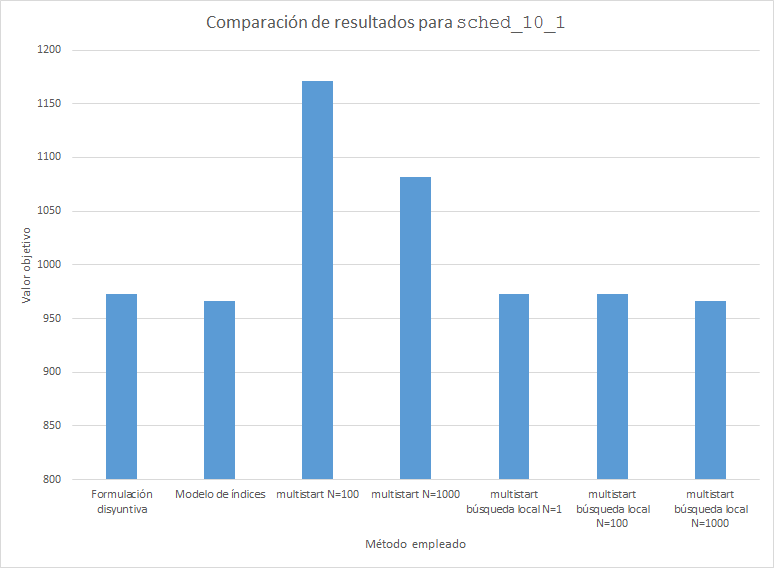
\includegraphics[width=1.0\textwidth]{comparacion_sched_10_1.png}
    \caption{Comparación de los resultados obtenidos para el fichero \texttt{sched\_10\_1.dat}}
\end{figure}

Comenzando por los métodos exactos, en todos los resultados obtenidos, el modelo de índices suele dar una solución mejor que la formulación disyuntiva, lo cual indica que los modelos de índices se ven afectados en de menor manera por el límite de tiempo de 100 segundos que se había impuesto inicialmente, y por ello en este caso son preferibles ya que encuentra mejores soluciones en un tiempo menor.\\

Respecto a los métodos heurísticos, los métodos \textit{multistart} aleatorizados en general dan malas soluciones incluso poniendo un número de iteraciones $N$ muy elevado. Por otro lado, si comparamos los resultados obtenidos por los métodos \textit{multistart} aleatorizados con búsqueda local, se puede observar como en general, el número de iteraciones $N$ no afecta demasiado a los resultados, puesto que en la mayoría de los problemas se obtiene el mismo resultado con ${N=}$ 1, 100 o 1000, además de que con solo una iteración, normalmente se obtienen resultados similares a los de los métodos no heurísticos. Por contra, la desventaja que tiene este método de búsqueda local es su tiempo de ejecución, el cual en ficheros con un elevado número de tareas es excesivo.
\end{document}
